\section{Deep Reinforcement Learning - Theorie}\label{hauptabschnitt_3}
Das wissenschaftliche Feld des maschinellen Lernens bietet viele verschiedene Ansätze einem Agenten beizubringen, wie er eine gegebene Aufgabe bewältigt. Dieses Feld lässt sich in drei Gruppen einteilen: Supervised Learning, Unsupervised Learning und \emph{Reinforcement Learning} (RL). RL differenziert sich von den anderen beiden Feldern durch die fehlenden Trainingsdaten. In diesem Feld werden die Trainingsdaten mittels Interaktionen in einem Environment gesampled. RL ist ein facettenreiches Forschungsfeld. Es vereint Anwendungen aus bspw. der Kontrolltheorie, dem maschinellen Lernen und weiteren Feldern in Einem. RL ist inspiriert durch den Ansatz des verstärkenden Lernens der Verhaltenspsychologie. Im Folgenden werden die für diese Arbeit benötigten Grundlagen eingeführt.


\subsection{Markov Decision Process}\label{absch_RL_mdp}
Der \emph{Markov Decision Process} (MDP) \cite{mdp_bellman} stellt ein mathematisches Framework für das Problem des Lernens durch Interaktion dar. 
Das Framework stellt die Rahmenbedingungen, in einem diskreten, stochastischen und sequenziellen Environment zielorientierte Entscheidungen zu treffen. Hierzu wird die gesamte Interaktion zwischen dem Agenten und dem Environment auf drei Signale reduziert. Ein \emph{State} ist hierbei der Zustand des Environments und beschreibt alle Übergangswahrscheinlichkeiten. Der Agent fällt seine Entscheidung auf Basis dieses States. Mittels \emph{Actions} kann der Agent mit dem Environment interagieren und dessen State verändern. Für die Ausführung einer Action erhält der Agent einen \emph{Reward} und den nächsten State. Der Reward stellt die Belohnung dar und kann sowohl positiv als auch negativ sein. Das Ziel des Agenten ist es, möglichst zielführende Actions auszuwählen und damit seinen Reward zu maximieren.

Dieser Prozess ist eine Erweiterung des \emph{Markov Reward Process} um die Fähigkeit Entscheidungen zu treffen. MDPs bieten die Möglichkeit Entscheidungen selbst in Situationen zu treffen, in denen der Ausgang nicht zu 100 \% von den Aktionen des Agenten abhängt, sondern durch Zufall verfälscht wird. Dem Agenten steht dabei die Teilmenge $A(s) \subset A $, die Menge aller möglichen Aktionen in State $s \in S$ zur Verfügung. Eine generelle Formulierung eines MDP deckt die meisten RL-Probleme ab und besteht aus dem folgenden Tupel $\langle S, A, P, R, \gamma \rangle$: 

\begin{itemize}
  \item $S$ ein Set aus States 
  \item $A$ ein Set aus Actions
  \item $P$ Übergangswahrscheinlichkeiten $P_{ss'}^a = \mathbb{P}[s_{t+1} = s' | s_t = S, a_t = A]$
  \item $R$ eine Reward-Funktion $R_s^a = \mathbb{E}[R_{t+1} | s_t = S, a_t = A]$
  \item $\gamma$ ein Diskontierungsfaktor $\gamma \in [0,1]$
  \begin{itemize}
     \item $\gamma$ = 0 => Monte-Carlo (Aktionswahl nur anhand des aktuellen States)
     \item $\gamma$ = 1 => $TD(1)$ (Aktionswahl anhand aller möglichen Folgestates)
  \end{itemize}
 % \item $Q(s,a)$ Action-Value Function $Q_{\pi}(s,a) = \mathbb{E}[G_t | S_t = s, A_t = a]$
  \label{lst:itemList_mdp}
\end{itemize}

\begin{figure}[htb]
 \centering
 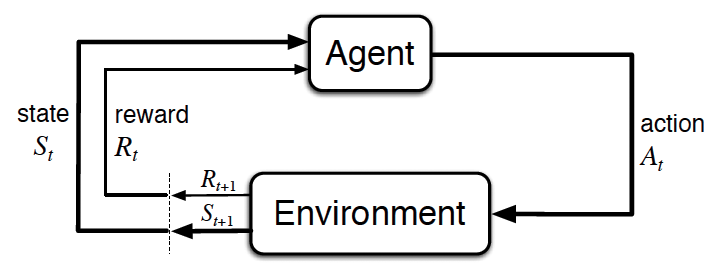
\includegraphics[width=0.3\textwidth,angle=0,scale=2.5]{abb/mdp_EnvLoop}
 \caption[Beschreibung]{Visualisierung des RL Prozesses mittels eines MDP \cite{sutton2011reinforcement}~[S.38]}
\label{fig:fig_mdpEnvLoop}
\end{figure}

Abbildung \ref{fig:fig_mdpEnvLoop} beschreibt die Interaktionen in einem MDP. Der Agent interagiert mit dem Environment für eine diskrete Anzahl an Schritten $t = 1, 2, 3, ..$. Am Anfang eines jeden Schrittes $t$ wählt der Agent eine Aktion $a_t$ und erhält daraufhin einen nummerischen Reward $R_{t+1} \in R \subset \mathbb{R}$ und den Folgestate $s_{t+1}$.

Während man im Markov Reward Prozess versucht die Action-Value Function $ Q_*(a) $ einer jeden Action zu schätzen, berechnet man in einem MDP die State-Action Value Function $ Q_*(s,a) $ einer jeden Action in jedem State oder man schätzt den Value eines States $ V_*(s) $. Bei der Berechnung des Values mittels $ V_*(s) $, wird eine optimale Auswahl der Actions vorausgesetzt. Ein Sternchen im Index steht hier repräsentativ für die optimale Policy. Der Index der Funktionen $ V_{\pi} $ und $Q_{\pi}$ referenziert folgend auf die aktuell verfolgte Policy. Die State-Value Function $V$ kann dabei als Dekomposition, in Form eines Erwartungswerts des aktuellen Rewards $ R_{t+1} $ und des diskontinuierten Values des Folge-States $ V(s_{t+1}) $, formuliert werden.


\begin{quotation}
\centering
   \( V_{\pi}(s) = \mathbb{E}_{\pi} [ R_{t+1} + \gamma V_{\pi}(S_{t+1}) | s_t = S ]  \) 
\end{quotation}


Die State-Action-Value Function $Q$ kann auf ähnliche Weise formuliert werden. Diese Funktion schätzt, wie gut eine Action $a$ unter der Prämisse ist, dass der Agent sich im State $ s_t $ befindet. 


\begin{quotation}
\centering
   \( Q_{\pi}(s,a) = \mathbb{E}_{\pi} [ R_{t+1} + \gamma Q_{\pi}(S_{t+1}, A_{t+1}) | s_t = S, a_t = A ]  \) 
   \label{eq:q_estimate}
\end{quotation}


Das Verhalten des Agenten kann, innerhalb des durch den MDP gegebenen Rahmens, als Policy $\pi(a|s)$ definiert werden, wobei $\pi $ eine Wahrscheinlichkeitsverteilung über alle States mit allen Actions darstellt. Diese Verteilung kann wie folgt definiert werden: 


\begin{quotation}
\centering
\( \pi(a|s) = \mathbb{P}_{t}[a_t = A | s_t = S] \label{eq:mdp_policy} \). %\footnote{Silver, vgl. \cite{silverCourse_mdp}~[S.26]}
\label{eq:mdp_policy}
\end{quotation}


Das beste Verhalten für ein gegebenes Problem  zu finden, bedeutet analog die Policy $\pi$ zu finden, die den Erwartungswert des akkumulierten diskontinuierten Rewards, über die Schritte $t$ hinweg, maximiert. Der Return $G_t$ ist der totale, diskontinuierte Reward und wird durch die folgende Gleichung definiert:

\begin{quotation}
\centering
   \( G_t = R_{t+1} + \gamma R_{t+2} + \gamma^{2} R_{t+3} + ... = \sum\limits_{k=0}^{\infty} \gamma^k R_{t+k+1} \) \footnote{Sutton und Barto, vgl. \cite{sutton2011reinforcement}~[S.44] } \label{eq:mdp_return}.
\end{quotation}


%$\mathbb{R} \rightarrow$ [0,1] mit $F(t) = P (X \le t)$ heißt Verteilungsfunktion von $X$



\subsection{Deep Learning}\label{absch_RL_deepL}
Im Gegensatz zu einem \emph{Single Layer Perceptron} (SLP), enthält ein \emph{Multi Layer Perceptron} (MLP) verborgene Schichten zwischen der Eingabe- und der Ausgabeschicht. Die verborgenen Schichten sind die sogenannten Hidden-Layers, von denen es beliebig viele hintereinander geben kann. Die Anordnung von mehreren Hidden-Layers von Neuronen, ist inspiriert vom biologischen Informations-Verarbeitungs-Prozess des menschlichen Gehirns. Da die verborgenen Layers nicht direkt mit der Ausgabe zusammenhängen, werden sie Hidden-Layer genannt \cite{Goodfellow-et-al-2016}[S. 164-165]. 

Ein Deep Neural Network (DNN) zielt darauf ab, Schicht für Schicht, aus einfachen Inputs wie bspw. einem Vektor aus Zahlen oder einem Pixel-Stream, informative Features zu extrahieren. Abbildung \ref{fig:maucher_dnn} zeigt eine abstrakte Darstellung eines DNN. Was ein einfaches MLP von einem vollwertigen DNN differenziert ist die Extraktion der Features (orange in Abb. \ref{fig:maucher_dnn}), die im Deep Learning dem Netzwerk überlassen ist. Diese Features müssen somit nicht manuell extrahiert werden. Der blaue Teil der Abbildung (\ref{fig:maucher_dnn}) ist applikations-spezifisch und könnte statt einem Classifier bspw. durch ein Regressionsmodell ersetzt werden. Die automatisierte Feature Extraction ermöglicht es eine Architektur auf unterschiedliche Probleme anzuwenden. Das ist möglich, da kein domänen-spezifisches Vorwissen mehr nötig ist, um dem applikations-spezifischen Teil des Netzwerks informative Features bereitzustellen. Die Verbindungen zwischen den Neuronen der jeweiligen Layer sind, wie bei einem SLP oder einem MLP, gerichtet und gewichtet. In der Feature Extraction befinden sich typischerweise Layer wie Convolutional-, Pooling-, RNN-, LSTM- und Attention-Layers. Der Teil des Classifier wird oft mit einem einfachen SLP oder einem mehrschichtigen MLP realisiert, bestehend aus Dense-Layers oder Fully-Connected-Layers.
\begin{figure}[htb!]
 \centering
 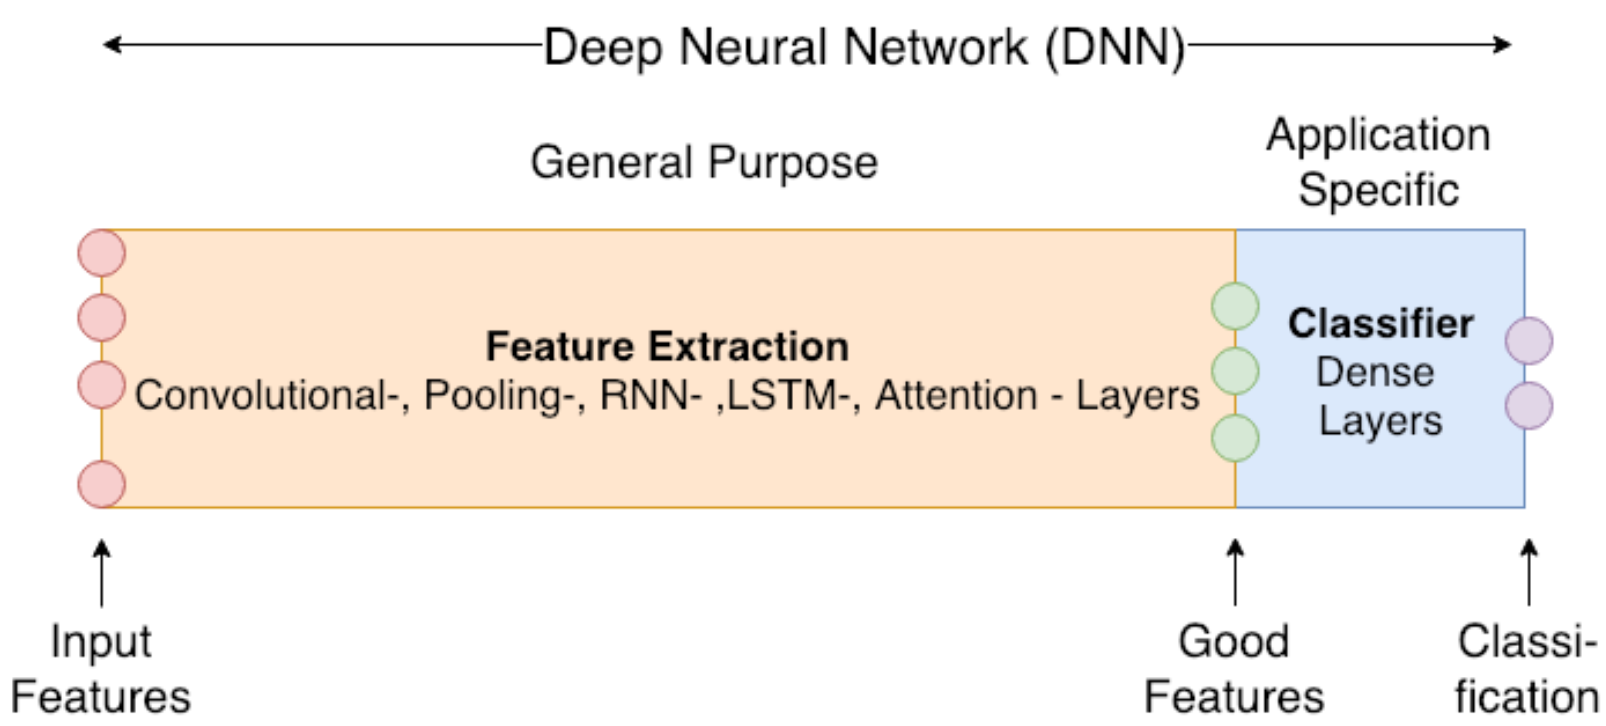
\includegraphics[scale=0.34]{abb/maucher_dnn}
 \caption[Beschreibung]{Abstrakte Darstellung eines DNN \cite{maucher_nb_cnn}. }
\label{fig:maucher_dnn}
\end{figure}
\newline

Viele Problemstellungen, wie das Verarbeiten eines Pixel-Streams, sind sehr komplex. Ein Frame eines Spiels von 60 auf 60 Pixeln, aufgeteilt in drei Farbkanäle, ergibt eine Anzahl von 10.800 Datenpunkten, die verarbeitet werden müssen. Anders als bei einem einfachem SLP oder einem MLP werden beim Deep Learning Entscheidungen nicht direkt abhängig vom Input getroffen. Hier werden über mehrere Abstraktions-Layer hinweg, nicht-lineare Anpassungen an den Daten vorgenommen. Eine ausführliche Motivation für tiefe Architekturen gibt die Arbeit \cite{bengio2009learning} von Yoshua Bengio.

Aufgrund der großen Anzahl an Neuronen sind die tiefen Neural Networks (NN) in der Lage komplexe Problemstellungen, wie aus einem Pixel-Stream eine Action abzuleiten, die in dieser Situation Reward-steigernd erscheint, auszuwählen. Im Bereich Deep Q-Learning wird bspw. die Approximation der State-Action-Value Function $Q(s,a)$, mit einem NN realisiert. Das State-Action-Value NN approximiert dann bspw. im Training den erwarteten durchschnittlichen Reward des übergebenen States-Action Tupels $(s,a)$ und wird typischerweise anhand des TD-Errors \ref{TD-Error} oder des Mean-Squared-Errors (MSE) \footnote{\label{foot:absch_RL_deepL_mse} Der MSE ist die Summe, der quadrierte Differenz zwischen tatsächlichen Wert $x(i)$ und der Vorhersage $\hat{x}(i)$ , geteilt durch die Anzahl an Datenpunkten. $MSE =  \frac{1}{n} \sum \limits_{i=1}^n ( x( i ) - \hat{x}(i))^2 $ } zum tatsächlich erhaltenen Return hin korrigiert. 



\subsubsection{Deep Feedforward Netzwerke}\label{absch_RL_deepL_FFN}
Deep \emph{Feedforward Networks} (FFN) sind die Basis des Deep Learnings. Ziel einer solch tiefen Architektur ist es, eine Funktion zu approximieren. So mapped ein solches Netzwerk, im Falle eines Classifiers, ein Eingabebild $x$ zu einem Label $y$. Das Mapping von Bild zu Label ist definiert durch $y = f(x,w)$, wobei $w$ die Gewichte darstellt, die es zu lernen gilt. Diese werden optimiert, um die bestmögliche Approximation von $f(x)$ zu ermöglichen. Der Name der FFN definiert den Informationsfluss. So haben FFNs, im Vergleich zu bspw. rekurrenten Netzwerken, ausschließlich vorwärts gerichtete Verbindungen - daher die Bezeichnung feedforward. Diese Grundarchitektur stellt die Basis vieler Anwendungen, wie CNNs dar. CNNs sind lediglich eine spezielle Form eines FFNs. Solche Netzwerke werden durch azyklische Graphen beschrieben, welche definieren, wie die approximierende Funktion zusammengesetzt ist. Hat man bspw. ein Netzwerk mit drei Schichten, so besteht dieses aus drei verschiedenen Funktionen, die wie folgt miteinander verkettet sind: 

\begin{quotation}
\centering
   \( f(x) = f^3 (f^2 ( f^1 (x))) \)
\end{quotation}

In diesem Fall stellt $f^1$ den ersten Layer dar, $f^2$ den zweiten, usw. Die gesamte Länge der Verkettung gibt die Tiefe des Netzwerks an. Der letzte Layer ist mit dem Output des Netzwerks verbunden. Ein repräsentatives Bild der Verkettung in Form eines MLP der Tiefe $L=3$ kann dem Anhang entnommen werden (\ref{anh_mlp_L3}). Die Eingabeschicht wird hierbei nicht zur Tiefe des Netzwerks gezählt. 

Während des Trainings werden die Parameter des gesamten Netzwerks so verändert, dass sich die Funktion $f(x)$ an die optimale Approximation $f_*(x)$ annähert. Jedes Element des Trainings $x$ muss also im Output-Layer möglichst genau das korrekte Label $y$ produzieren. Wie die Layer zwischen Input und Output korrigiert werden, um näher an $f_*(x)$ zu gelangen, wird über den angewandten Lernalgorithmus definiert.

Eine tiefe FFN-Architektur könnte wie folgt sein: Am Netzwerk liegt der Input, bspw. ein eindimensionaler Vektor, an. Dieser Vektor wird dann durch eine Serie an Hidden-Layers, bis hin zum Output-Layer transformiert. Jeder Hidden-Layer besteht aus mehreren Neuronen, die vollständig mit den Neuronen des vorherigen und nachfolgenden Layers verbunden sind. Neuronen in Hidden-Layers teilen hier keine Verbindungen untereinander und agieren unabhängig voneinander. Der eben beschriebene Teil der Architektur übernimmt die Feature Extraction. Der letzte vollständig verbundene Layer entspricht dem Output-Layer. Im Fall von Klassifikationen würden im Output-Layer die Scores für die jeweiligen Klassen stehen, bspw. 10 Outputs bei 10 verschiedenen Klassen. 



\subsection{Convolutional Neural Networks}\label{absch_RL_convNets}
CNNs sind seit mehreren Jahren etabliert im Einsatz für Objekt-Detektion, Objekt-Erkennung, Sprach-Erkennung und weitere. Diese Netzwerke sind eine spezialisierte Form der in Unterkapitel \ref{absch_RL_deepL_FFN} vorgestellten FFNs. Ebenso wie FFNs bestehen CNNs oft aus sehr vielen Schichten an Neuronen, mit Gewichten, die es zu lernen gilt. Der größte Unterschied zwischen FFNs und CNNs besteht in der Verwendung der Convolutional-Layer bzw. in der Anwendung von Convolutional Filtering. Diese Layer sind darauf ausgelegt lokale Informationen, bspw. aus benachbarten Pixeln aus Bildern oder umgebenden Wörtern in einem Text in ein Feature zu extrahieren. Aufbauend auf der Annahme, dass die umgebende Region für eine betrachtete Stelle relevant ist, teilen sich die Neuronen dieser Region die Gewichte zum nachfolgenden Neuron. Durch die many-to-one-Beziehung sind CNNs in der Lage, komplexe Inputs wie ein Bild zu verarbeiten. CNNs lernen damit automatisch häufig vorkommende Merkmale der Trainingsdaten, welche für den applikations-spezifischen Teil der Architektur relevant sind. 
 
Die Bilder des Datensatzes \emph{CIFAR-10} \footnote{\label{foot:absch_RL_CNN_CIFAR10} Der Datensatz von CIFAR-10 beinhaltet 60.000, $32*32$ Farbbilder, eingeteilt in 10 Klassen.} \cite{cifar10_krizhevsky} sind bspw. $32*32$ Pixel groß und haben drei Farbkanäle (RGB). Damit hat der ersten Convolutional-Layer einen Input von $32*32*3 = 3.072$ Datenpunkten. Im Fall dieser Arbeit wird bereits mit doppelt so großen Frames, ebenfalls mit drei Farbkanälen gearbeitet ($64*64*3 = 12.288$). Auch diese Größe ist noch weit von einem brauchbaren Bild entfernt, wie Abbildungen \ref{fig:pic_chaserGros} und \ref{fig:pic_chaserKlein} zeigen. Eine einfache FFN-Architektur benötigt für ein solches Bild, je nach Aufbau, sehr viele Gewichte und ist deshalb ungeeignet, um direkt mit solchem Input zu interagieren. Convolutional-Layer verbinden Regionen von Neuronen des vorangegangenen Layers mit einem Neuron des Convolutional-Layers. Diese Layer bieten durch die Feature Extraction aus Regionen eine effiziente Reduktion des vorangegangenen Layers. Eine Veranschaulichung dieses Konzepts bezüglich des Netzwerks, bei zweidimensionalem Input, ist im Anhang gegeben (\ref{anh_conv2d}).

CNNs für die Farbbild-Verarbeitung haben im Unterschied zu FFNs, ebenso wie ihr Input, einen dreidimensionalen Aufbau - die Neuronen werden in Höhe, Breite und Tiefe organisiert. Die Breite und die Höhe stehen hierbei für die räumlichen Informationen und die Tiefe für die Anzahl der Farbkanäle des anliegenden Bildes. So bestehen Convolutional-Layer in diesem Fall nicht aus einfachen Neuronen-Schicht, sondern aus einem dreidimensionalen Volumen an Neuronen. 

Typischerweise bestehen CNNs aus drei verschiedenen Layern: Convolutional-Layer, Pooling-Layer und Fully-Connected-Layer. Die einzelnen Layer sind folgend detaillierter erläutert. 


 % \item Input: Dieser ist im Fall von CIFAR-10 ein Bild der Größe $32*32$, mit drei Farbkanälen. 
\textbf{Convolutional:} Diese Layer berechnen den Output aus den lokalen Regionen des Inputs. Sei $(r \times c)$ der zweidimensionale Input, bspw. ein Schwarz-Weiß-Bild, wobei $r$ die X- und $c$ die Y-Koordinate eines Pixels angibt. So gibt $r*c$ die Größe des Bildes an. Weiter sei $(a \times b)$ ein Filter, mit der \emph{Kernel Size} $a*b$, wobei der Filter kleiner als der Input ist. Dieser Filter wird von oben links, bis unten rechts über den Input geschoben. Hierbei wird bei jeder Iteration das Skalarprodukt zwischen den jeweiligen Koeffizienten der Region des Inputs und den Koeffizienten des Filters errechnet. Dieses Skalarprodukt wird nach Anwendung der Aktivierungsfunktion $g$ in den folgenden Layer geschrieben. Ist der geschriebene Wert positiv bedeutet dies, dass das Feature, welches durch die verwendeten Filter repräsentiert wird, vorhanden ist. Ist der Wert $0$ kommt dieses Feature nicht an dieser Stelle des Inputs vor. Der \emph{Stride} entscheidet dabei wie weit der Filter nach jeder Operation bewegt wird. Bei einem Stride von $s=1$ ergeben sich $(r-a+1) * (c-b+1)$ mögliche Positionen für den Filter. Allgemein ist der Output im zweidimensionalen Fall von der Größe $[(r-a+s) \times (c-b+s)]$. Ein Bild dieses Ablaufs kann dem Anhang entnommen werden (\ref{anh_convConcept}). Dieses Bild zeigt einen Input der Größe $[10 \times 10]$ und einen Filter der Größe $[3 \times 3]$. Mit einem Stride von $s=1$ ergibt sich als Ausgabe dieser Operationen ein Layer der Größe $[8 \times 8]$ ($~[(10-3+1) \times (10-3+1)]~$). 
Der Stride des Filters kann auch größer als $1$ sein. Zudem gibt es die Option, dass man dem Bild ein sogenanntes \emph{Padding} hinzufügt oder nicht. Für das Padding gibt es wiederum selbst verschiedene Optionen für die Realisierung. Im Falle der Anwendung von Padding errechnet sich die Größe der Ausgabe bei der Größe des Padding $p$ und bei quadratischem Input und Filter wie folgt: 
\begin{quotation}
\centering
   \( p = \frac{r-a+2p}{s} + 1  \) 
\end{quotation}


\textbf{Pooling:} Ein Pooling-Layer komprimiert die Daten entlang der räumlichen Achsen. Ähnlich wie beim Convolutional-Layer gibt es beim Pooling-Layer eine Art Filter. Dieser Filter verschiebt sich um den Wert des Strides. Bei diesem Filter werden die betroffenen Elemente jedoch nicht aufsummiert, sondern die Koeffizienten, welche der Filter abdeckt, werden mit dem Max-Operator auf einen reduziert. So wird bspw. aus der Ausgabe eines Layers mit $[32 \times 32 \times 10]$, mittels eines Filters der Größe $[2 \times 2]$ und einem Stride von 2 die Ausgabe des Pooling-Layers mit $[16 \times 16 \times 10]$ erzeugt.

\textbf{Fully-Connected:} Dieser Layer errechnet die Scores für die jeweiligen Klassen. Im Fall von zehn Klassen ist das Resultat ein Volumen der Maße $[1 \times 1 \times 10]$ \footnote{Die Ausgabe des vorangehenden Layers wird typischerweise zu einem eindimensionalen Vektor gestaucht. So ergibt sich aus einen Layer der Größe $[2 \times 2]$ ein Vektor der Größe $[1 \times 4]$.}. Bis hier sind die räumlichen Informationen des Bildes vollständig transformiert und übrig bleibt ein quasi eindimensionaler Vektor mit den zehn Klassen-Scores des CIFAR-10 Datensatzes.

\textbf{Activation:} Die Funktion $g$ realisiert eine elementweise Aktivierungsfunktion auf den oben beschriebenen Skalarprodukten. 

Mögliche nicht-lineare Aktivierungsfunktionen der Neuronen: 
  \begin{itemize}
  	\item Sigmoid: $g(x) = \frac{1}{1+e^{-x}}$
  	\item Hyperbolischer Tangens: $g(x) = \frac{1- e^{-2x}}{1+e^{-2x}}$
  	\item ReLU: $g(x) = max(0,x)$ 
  	\item etc.
\end{itemize}


%\cite{krizhevsky2012ConvImageClass}
%\cite{yamashita2018convMedUse}
%CNN's s 




\subsection{Deep Reinforcement Learning}\label{absch_RL_deepRL}
In Deep Reinforcement Learning werden die Policy oder die State-Value Function oder beide zusammen mit einem tiefen NN realisiert. Das hat den Vorteil, dass bspw. das Mapping der State-Action-Value Function $Q$ beim Q-Learning nicht mehr in einer zweidimensionalen Tabelle gespeichert wird. Hier übernimmt das Mapping von State-Action Tupel zu Value ein tiefes NN. Das spart einerseits Anforderungen an die Hardware und kann andererseits schneller eine Antwort liefern, da keine mit der Problemgröße wachsende Tabelle durchsucht werden muss. 

\paragraph{on-policy vs. off-policy}\label{onVSoff-Policy}
Folgend wird der Unterschied zwischen \emph{on-policy}- und \emph{off-policy}-Verfahren erläutert. Beide Verfahren, sowohl \emph{on-policy}, wie auch \emph{off-policy} aktualisieren ihre Schätzungen der Q-Werte anhand des Tupels $(s',a')$. Der Folgestate ist $s'$ und die dann gewählte Action ist $a'$. Die Verfahren unterscheiden sich in der Annahme für die Wahl der folgenden Action $a'$ des Tupels. \newline
\textbf{on-policy:} Diese Verfahren gehen davon aus, dass die Action $a'$ mit der aktuell verfolgten Policy $\pi_t$, zum Zeitpunkt $t$ ausgewählt wird. SARSA ist bspw. ein on-policy-Verfahren.\newline
\textbf{off-policy:} Bei diesem Verfahren wird davon ausgegangen, dass die Action-Wahl \emph{greedy}\footnote{Eine greedy Wahl der Action nimmt immer die Action, welche den höchsten totalen geschätzten Reward verspricht.} getroffen wird. Aus diesem Grund ist Q-Learning ein off-policy Verfahren.

In on-policy geschehen Updates also anhand einer Action-Wahl der aktuell verfolgten Policy. In off-policy wird davon ausgegangen, dass die Action-Wahl einer greedy Policy folgt und somit nicht der aktuell verfolgten Policy entspricht.


\subsubsection{Function Approximation}\label{subsub:absch_RL_deepL_funcAppr}
Im Rahmen dieser Arbeit werden sowohl die Policy, als auch die Value Function mit einem tiefen NN approximiert. 

\paragraph{Value Function Approximation} 
Die State-Value Function $V$ mapped einen State $s$ auf einen Value. Das NN ist mit dem Vektor $w$ parametrisiert. $V(s,w)$ approximiert damit die tatsächliche State-Value Function $V_{*}(s)$. Typischerweise ist die Dimensionalität des Vektors $|w|$ geringer, als die Anzahl an möglichen States $|S|$. Die Reduktion des Problems von der Anzahl an möglichen States auf die Anzahl an verwendeten Gewichten ermöglicht das agieren in komplexen kontinuierlichen Environments. Das Netzwerk wird in Richtung des approximierten erwarteten Returns ($R_{t+1} + \gamma V(S_{t+1}$), bekannt als das \emph{TD Target}, korrigiert. Die Größe eines Updates von $V$ wird mittels des Hyperparameters $\alpha$ kontrolliert. 

\begin{quotation}
\centering
   \( V(s_t) \leftarrow V(s_t) + \alpha(R_{t+1} + \gamma V_{t+1} - V(s_t)) \) \\
\end{quotation} 
Ein Update der State-Action-Value Function $Q$ erfolgt analog. 

\begin{quotation}
\centering
   \( Q(s_t, a_t) \leftarrow Q(s_t, a_t) + \alpha(R_{t+1} + \gamma Q(s_{t+1}, a_{t+1}) - Q(s_t, a_t)) \) \\
\end{quotation}
 Der Estimator der State-Value Function ist wie folgt definiert:

\begin{quotation}
\centering
   \( V_w (s) = \mathbb{E}_{\pi} [ \sum\limits_{k = 0} \gamma^k R_{t+k+1} | s_t = S ] \) \footnote{Der Exponent k steht für die Anzahl der Episoden.}. \\
\end{quotation}
Der Iterator $k$ ist limitiert über die Anzahl an Schritten, die vorausgeschaut werden. Bei $TD(\lambda)$ gibt $\lambda$ diese Anzahl vor. Da man am Ende einer Episode den tatsächlich erhaltenen Reward vom Environment bekommt, ist dieser Teil ein Supervised Learning Problem und kann auch ebenso optimiert werden. 

\paragraph{Policy Approximation}
Policy Gradient Methoden zielen darauf ab, eine Policy direkt aus der Interaktion mit dem Environment zu modellieren und optimieren. Typischerweise wird die Policy ebenfalls als parametrisierte Funktion $\pi_{\theta}(a|s)$ mit den Parametern $\theta$ formuliert. Der resultierende Value der Objectiv Function ist somit abhängig von der verfolgten Policy $\pi$. Die Reward- bzw. Objectiv Function wird definiert durch folgende Gleichung:

\begin{quotation}
\centering
   \(\ J(\theta) = \sum\limits_{s \in S} d^{\pi_{\theta}}(s) V^{\pi_{\theta}}(s)  =  \sum\limits_{s \in S} d^{\pi_{\theta}}(s) \sum\limits_{a \in A} \pi_{\theta}(a|s) Q^{\pi_{\theta}}(s,a)   \) , \\
% Formel von 
% https://lilianweng.github.io/lil-log/2018/04/08/policy-gradient-algorithms.html#what-is-policy-gradient
\end{quotation}
wobei $d^{\pi}(s)$ die Verteilung der makrov'schen Kette für die Policy $\pi_{\theta}$ darstellt. Mittels des Gradienten Aufstiegsverfahrens wird $\theta$ in die Richtung gelenkt, die der Gradient $\bigtriangledown_{\theta}J(\theta)$ vorschlägt, um die erwarteten Rewards zu maximieren.

Das Policy Gradient Theorem legt das theoretische Fundament für die Umformung des Gradienten $ \bigtriangledown J(\theta) $ zu einem Estimator $\mathbb{E}$. \footnote{ Sutton und Barto geben in Sektion 13.2 \cite{sutton2011reinforcement}{S. 268} den Beweis für den episodischen Fall. }

\begin{quotation}
\centering
   \( \bigtriangledown J(\theta)  =  \mathbb{E}_{\pi_{\theta}} [ \bigtriangledown log \pi_{\theta}(a | s, \theta) Q^{\pi_{\theta}}(s,a) ] \) 
\end{quotation}

$ \pi_{\theta} $ ist eine stochastische Policy und $ Q^{\pi_{\theta}} $ ist der State-Action Value Funciton Estimator.


\paragraph{Advantage}\label{subsubsec_RL_advantage}
Um die Varianz im Training zu verringern, wird statt der lediglich value-based Methoden, häufig die Advantage Function eingesetzt und statt der Value Function im Policy Gradient verwendet \cite{schulman2017proximal}. 
Der Advantage ist definiert wie folgt: 

\begin{quotation}
\label{Advantage-Estimate}
\centering
   \(  A(s,a) = Q_b(s,a) - V_w(s)  \)
\end{quotation}

$ Q(s,a) $ entspricht dem Q-Value von Action $ a $ im State $s$, $ V(s) $ dem Value des States $ s $.  Ein Nachteil dieser Praxis ist, dass man $ Q $ und $ V $mit zwei unterschiedlichen Parameter-Sets trainieren muss. Dies geht aus den Indizes der vorangegangenen Gleichung hervor. Um die Notwendigkeit von zwei unterschiedlichen Parametrisierungen zu vermeiden, wird häufig die Umformung angewandt, welche den Advantage Function Estimator $ A $ durch einen Estimator des TD-Errors ersetzt. Für die tatsächliche Value Function $ V^{\pi_{\theta}}(s) $ definiert sich der TD-Error $ \delta^{\pi_{\theta}} $ folgendermaßen: 

\begin{quotation}
\label{TD-Error}
\centering
   \(  \delta^{\pi_{\theta}} = r + \gamma V^{\pi_{\theta}}(s') - V^{\pi_{\theta}}(s)  \)
\end{quotation}

Die Definition von $ Q(s) $ (\ref{eq:q_estimate}) entspricht dem aktuellen Reward, plus dem geschätzten, erwarteten und diskontinuierten Value des nächsten States $ s' $.  Der erste Teil des TD-Errors $ ( r + \gamma V^{\pi_{\theta}}(s') ) $, bedingt durch den aktuellen State $s$ und die Action $a$, entspricht somit der State-Action-Value Function $Q$. 
Ersetzt man nun die State-Action-Value Function mit dem ersten Teil des TD-Errors, für die Schätzung der Advantage Function, erhält man folgende Gleichung: 

\begin{quotation}
\centering
   \( \mathbb{E}_{\pi_{\theta}} [ \delta^{\pi_{\theta}} | s,a]  =  \mathbb{E}_{\pi_{\theta}} [ r + \gamma V^{\pi_{\theta}}(s') | s,a ] - V^{\pi_{\theta}}(s) \)
\end{quotation} 

Somit kann man den TD-Error verwenden, um den Policy-Gradienten zu schätzen und man umgeht damit die Notwendigkeit eines extra Netzwerks bzw. Parameter-Sets für $Q$. Da $V^{\pi_{\theta}}(s)$ den Value des aktuellen States repräsentiert, kann dieser Teil außerhalb des Estimators sein. Nun kann der TD-Error verwendet werden, um den Policy Gradienten zu berechnen.  

\begin{quotation}
\centering
   \(  \delta_{\theta}J(\theta)  =  \mathbb{E}_{\pi_{\theta}} [\bigtriangledown_{\theta} log \pi_{\theta}(s, a) \delta^{\pi_{\theta}}]  \)
\end{quotation}


\subsection{Actor Critic}\label{absch_RL_acModel}
Die Ansätze in model-free RL lassen sich grob in drei Gruppen einteilen.
  \begin{itemize}
  	\item Value-basierte Methoden (bspw. Q-Learning und Deep Q-Learning): In diesen Methoden lernt der Agent eine Value Function $V$, welche jedem State oder jedem State-Action Tupel einen Value zuweist. Diese funktionieren zuverlässig in einer Umgebung mit einer endlichen Menge an Actions bzw. States.
  	\item Policy-basierte Methode (bspw. REINFORCE Policy Gradient): Hier lernt der Agent direkt eine Policy $\pi$, ohne dabei eine State-Value Function zu nutzen. Diese Methoden sind besonders stark in Bereichen, in denen das Environment einen stochastischen oder kontinuierlichen Action Space aufweist.
  	\item Hybrid Methoden (Actor Critic): Diese Methodik vereint die zuvor erwähnten Ansätze zu einem, welcher sowohl eine Value Function einsetzt als auch eine Policy verwendet. Aufgeteilt auf zwei NNs approximiert der Critic eine Value Function, welche den Aktor korrigiert. Diese Methodik vereint die Vorteile der beiden vorherigen Ansätze. Das Training eines Actor Critic Modells generiert seine Samples typischerweise on-policy (\ref{onVSoff-Policy}). Im Fall einer synchronisierten Batched \emph{Advantage Actor Critic} (A2C) Implementierung generiert der Aktor eine Anzahl an Samples $T$, wobei $T$ deutlich kleiner als die Episodenlänge ist. Daraufhin evaluiert der Critic die Samples, aktualisiert seine Schätzungen für die Values der jeweiligen States und aktualisiert die Policy des Aktors.
  \end{itemize}
In dieser Arbeit wird das Actor Critic Modell verwendet. 

%\subsubsection{Advantage}\label{subsubsec_RL_advantage}




\subsection{Proximal Policy Optimization}\label{absch_RL_ppo}
Der Proximal Policy Optimization (PPO) \cite{schulman2017proximal} Algorithmus ist ein on-policy (\ref{onVSoff-Policy}) Policy Gradient Algorithmus. Im folgenden Unterkapitel wird der in dieser Arbeit verwendete Algorithmus zur Optimierung der Policy vorgestellt. 

Unabhängig von den in dieser Arbeit erwähnten Problemen in RL (\ref{absch_EXP_procgen} Overfitting auf große Datensätze, \ref{par:durch_EXP_vgl_200_unbeschr} Sparse-Reward-Problem), haben on-policy Policy Gradient Methoden oft zwei weitere generelle Probleme. Einerseits besteht das Problem, dass generierte Samples bzw. Batches immer abhängig von der aktuell verfolgten Policy sind. Dadurch erlebt der Agent sich konstant ändernde State- und Reward-Verteilungen, was zu Instabilität im Training führen kann.
Andererseits besteht in RL eine große Sensitivität gegenüber Hyperparameter Tuning. 

Darüberhinaus besteht in RL allgemein die Gefahr zu großer Policy-Updates. Wird bspw. ein Batch, anhand dessen die Policy optimiert werden soll, unter einer zufällig schlechten Policy gesampled, so kann es passieren, dass sich die Policy mit einem Update sehr weit von der aktuell verfolgten Policy $ \pi_{\theta} $ entfernt. Auch wenn die Policy bisher zu keinen schlechten Ergebnissen geführt hat, werden nun ggf. sehr viele gute Eigenschaften der bestehenden Policy revidiert. Daraufhin wird der nächste Batch unter noch schlechteren Umständen gesampled. Solch eine falsche Korrektur der Policy zu kompensieren, kann viele Zeitschritte im Training kosten und ggf. erholt sich die Policy nicht mehr vom ersten Batch, der die Policy in diese Richtung verbessert bzw. verschlechtert hat. Das PPO-Paper \cite{schulman2017proximal} zeigt in Abschnitt $6.1$ Experimente mit unbeschränkten Policies. Diese Experimente liefern einen empirischen Beweis für Schwierigkeiten mit unbeschränkten Updates.

\subsubsection{Hintergrund}\label{absch_RL_PPO_hintergrund}
Der PPO Algorithmus ist maßgeblich durch den Trust Region Policy Optimization (TRPO) Algorithmus \cite{schulman2015trust} inspiriert. 

\paragraph{Trust Region Policy Optimization}\label{par:absch_RL_PPO_hintergrund_TRPO}
Um die Stabilität im Training zu verbessern, verhindert TRPO unter anderem die zuvor erwähnten, zu großen Policy Updates. TRPO löst dieses Problem mittels eines sogenannten \emph{KL-Divergence Constraint}, in der Objectiv Function. Grundsätzlich versucht der Algorithmus Folgendes zu maximieren: 

\begin{quotation}
\centering
   \( L^{TRPO}(\theta) =  \mathbb{E}_t [ \frac{ \pi_{\theta}(a_t | s_t)}{ \pi_{\theta_{old}}(a_t | s_t) } A_t  -  \beta KL [ \pi_{\theta_{old}}( \cdot | s_t), \pi_{\theta}( \cdot | s_t ) ] ] \).
\end{quotation}

Der Teil der Gleichung links ($(\pi_{\theta} / \pi_{\theta_{old}}) A_t$) ist ein Verhältnis zwischen der neuen und der alten Policy, unter Betrachtung desselben State-Action Tupels, multipliziert mit dem Advantage Estimate. Dieser Teil stellt die unbeschränkte Policy-Optimierung. Der Hyperparameter $ \beta$, stellt den sogenannten Penalty Coefficient dar. Dieser entscheidet wie stark das KL-Divergence Constraint beachtet wird. Je größer $ \beta$, desto kleiner ist das resultierende Update. Der Term $ KL [ \pi_{\theta_{old}}( \cdot | s_t), \pi_{\theta}( \cdot | s_t ) ] $  \footnote{Kullback-Leibler-Divergence: $ D_{KL}(\pi_1 || \pi_2)[s] = \sum_{a \in A} \pi_1 (a|s) log \frac{\pi_1 (a|s)}{\pi_2 (a|s)} $} errechnet die Divergenz zwischen der alten und der neuen Policy, in anderen Worten die Entfernung zwischen den zwei Policies. Dies geschieht unter Betrachtung des States $s_t$ und allen möglichen Actions.

\subsubsection{PPOs Clipped Objectiv Funciton}\label{absch_RL_qFunc}
Sei $ r_t(\theta) $ das Verhältnis der Wahrscheinlichkeitsverteilungen $ \pi_{\theta} / \pi_{\theta_{old}} $, sodass $ r_t(\theta_{old}) = 1 $, so beschreibt $ r_t(\theta) A_t $ das unbeschränkte TRPO Objectiv. 

\begin{quotation}
\centering
   \( L^{CPI}(\theta) =  \mathbb{E}_t [ \frac{ \pi_{\theta} (a_t | s_t) }{ \pi_{\theta_{old}} (a_t | s_t) } A_t ] = \mathbb{E}_t [ r_t(\theta) A_t ] \)
\end{quotation}

CPI referenziert hier auf \emph{Conservative Policy Iteration} der Arbeit \cite{kakade2002approximately}. Das unbeschränkte TRPO Objectiv wurde in dieser Arbeit erstmalig vorgestellt. Somit ist $ r_t(\theta) $ größer als $ 1 $, wenn eine Action unter der neuen Policy wahrscheinlicher ist, als unter der alten Policy. Im umgekehrten Fall ist $ r_t( \theta ) $ kleiner als 1. Wie in der letzten Problematik \ref{par:absch_RL_PPO_hintergrund_TRPO}im zweiten Absatz bereits erklärt, kann auch dieses Objectiv zu sehr großen Policy Updates führen. Das Update kann so groß sein, dass die Policy es eventuell nicht mehr kompensieren kann, falls es ein schlechtes Update war. 

PPO greift das Objectiv von TRPO auf, doch beschränkt es sich nicht auf die aufwendig zu berechnende KL-Divergence, sondern clipped es lediglich um den Wert $ 1 \pm \epsilon $. $ \epsilon $ ist ein Hyperparameter, welcher typischerweise $0,2$ ist. Zusammen mit dem Min-Operator kann nun das eigentliche PPO-Objectiv vorgestellt werden. 

\begin{quotation}
\label{PPO-clip-objective}
\centering
   \( L^{CLIP}(\theta) =  \mathbb{E}_t [ min ( r_t(\theta) A_t , clip ( r_t(\theta), 1 + \epsilon, 1 - \epsilon ) A_t ) ] \)
\end{quotation}

Diese Objectiv Function nimmt das Minimum aus zwei Termen. Der erste Term im Min-Operator ($ r_t(\theta) A_t $) ist das unbeschränkte TRPO Objectiv, wie in \ref{absch_RL_PPO_hintergrund} vorgestellt. Der zweite Term beschränkt das Verhältnis $ r_t(\theta) $ auf eine Differenz von $1 \pm \epsilon $ und multipliziert dann mit dem Advantage Estimate, wie in \ref{absch_RL_actorCriticPPO} definiert. Die daraus resultierende Policy $\pi_{\theta}$ kann sich somit, innerhalb eines Updates, nicht weiter als $ \epsilon $ von der alten Policy $ \pi_{\theta_{old}} $ entfernen. 

Der PPO Algorithmus vereinfacht somit das KL-Divergence Constraint zu einer Clip-Operation. Zudem ist eine Schwäche des TRPO, dass es kein $ \beta $ gibt, welches über mehrere Environments hinweg erfolgreich ist. Selbst in einem einzigen Environment kann ein statisches $ \beta $ zu einer schlechten Performance führen. Dieses Problem besteht bei PPO nicht. 

%EVTL INTUITION HINTER DER GLEICHUNG ERKLÄREN. AUCH DIE GRHEN IM PPO PAPER FÜR DEN ADVANTAGE...


\subsubsection{PPO Actor Critic Style}\label{absch_RL_actorCriticPPO}
In dieser Arbeit wird der PPO Algorithmus zusammen mit dem Actor Critic Model verwendet. Folgend wird der \emph{Loss}-Term vorgestellt, welche PPO einsetzt. Im PPO-Paper teilen sich die Netzwerke für die Value Function und die State-Action-Value Function einen großen Teil der Parameter. Genauer teilen sie sich die Object Detection und Feature Extraction. 

In dieser Arbeit sind die Object Detection und Feature Extraction durch das IMPALA-Netzwerk (\ref{absch_setup_impala}) gegeben. Die Architektur teilt sich im Output-Layer in zwei Heads auf. Einen für die Value Function und einen für die Policy. Aufgrund dessen, dass sich die NNs einen großen Teil der Netzwerk-Parameter teilen, kann die gesamte Architektur mittels einer Loss-Term optimiert werden. 

\begin{quotation}
\centering
   \( L_t ^{CLIP+VF+S}(\theta) =  \mathbb{E}_t [L_t ^{CLIP}(\theta) - c_1 L_t ^{VF}(\theta) + c_2 S[\pi_{\theta}](s_t) ] \)
\end{quotation}

Der Term $ L_t ^{CLIP}(\theta) $ stellt dabei das Clipped Objectiv dar, wie in \ref{PPO-clip-objective} definiert. $ L_t ^{VF}(\theta) $ stellt einen Loss-Term dar, welche wie folgt definiert ist:
\begin{quotation}
\centering
   \(  L_t ^{VF}(\theta) = (V_{\theta}(s_t) - V_t ^{targ})^2  \) .
\end{quotation}

$V_{\theta}(s_t)$ ist eine Value Function, wie sie im Abschnitt \ref{subsub:absch_RL_deepL_funcAppr} definiert ist. $V_t ^{targ}$ ist der tatsächliche Return eines Batches. Dieser Term $ L_t ^{VF}(\theta) $ ist somit ein Squared-Error Loss. 

$ S[\pi_{\theta}](s_t) $ ist ein Term, welcher die Entropie der Gleichung erhöht. Durch den Entropie-Term betreibt der Agent im Training anfänglich viel Exploration, bis die anderen Terme der Gleichung ausreichend Gewicht erlangen. Die Koeffizienten $c_1$ und $c_2$ sind Hyperparameter zur Gewichtung der jeweiligen Terme. Optimiert wird dann mit einem stochastischen Gradienten-Abstiegsverfahren.

Der PPO Algorithmus nutzt eine Implementierung, wie sie in \cite{mnih2016asynchronous} dargestellt ist. In dieser Implementierung sampled die Policy für $ T $ Schritte, wobei $T$ deutlich kleiner als die Episodenlänge ist. Anhand dieses Segments wird der Agent aktualisiert. Diese Art des Samplings benötigt jedoch eine Anpassung des Advantage Estimators, da dieser ansonsten Teile der \emph{Trajectory}. Eine Trajectory $\tau_H$ ist ein Pfad des Agenten durch den State Space des Environments bis zum Horizont $H$ beachten würde, welche über T hinaus liegen. Das kleine $t$ spezifiziert hier den aktuellen Zeitschritt in $[0,T]$ und das große $T$ spezifiziert die Länge des Segments. 

\begin{quotation}
\centering
   \( A_t = -V(s_t) + r_t + \gamma r_{t+1} + ... + \gamma^{T-t+1} r_{T-1} + \gamma^{T-t} V(s_T) \)
\end{quotation}

Im Fall von $\lambda = 1$ kann die vorangegangene Gleichung zur folgenden Gleichung vereinfacht werden. $\delta_{t}$ entspricht hierbei dem TD-Error zum Zeitpunkt $t$, wie in \ref{TD-Error} definiert.

\begin{quotation}
\centering
   \( A_t = \delta_t + (\gamma \lambda)\delta_{t+1} + ... + (\gamma \lambda)^{T-t+1} \delta_{T-1} \)
\end{quotation}

\paragraph{Pseudocode PPO}
Die Implementierung des PPO, welcher mit Segmenten von Trajectories konstanter Länge arbeitet, ist folgend als Pseudocode gegeben. Dieser Code geht von einem Fall aus, in welchem man mehrere Aktoren parallel laufen lässt und dann über die Segmente aller Aktoren optimiert. In dieser Arbeit wird jedoch nur mit einem Aktor gearbeitet ($N=1$). 


\begin{algorithm}
\caption{Pseudocode Implementierung des PPO, Actor Critic }
\begin{algorithmic}

\WHILE{$i < iterations $}
	\WHILE{$actor < N$}
		\STATE  run policy $ \pi_{\theta_{old}} $ in environment for T steps 
		\STATE compute advantage estimates $ A_1, ..., A_T$
	\ENDWHILE
	\STATE optimize surrogate objectiv $ L(\theta) $ with K epochs and minibatches of size $ M \leq NT $
	\STATE $ \theta_{old} \leftarrow \theta $
\ENDWHILE

\end{algorithmic}
\end{algorithm}


\subsection{IMPALA Architektur}\label{absch_setup_impala}
Die IMPALA-Architektur wird im Paper \cite{espeholt2018impala} erstmalig vorgestellt. Die Abkürzung IMPALA steht für \textbf{Imp}ortance Weighted \textbf{A}ctor-\textbf{L}earner \textbf{A}rchitecture. Der wichtigste theoretische Beitrag dieses Papers besteht in der Vorstellung einer Möglichkeit zur asynchronen Separation von Aktoren und Lernern. Das ermöglicht es mehreren Aktoren simultan auf unterschiedlichen Maschinen, mit unterschiedlichen Versionen derselben Policy zu trainieren. Nach einer gewissen Anzahl von Episoden schickt der Aktor seine Samples an den Lerner. Der Lerner muss daraufhin, während des Updates, in Betracht ziehen, dass die Samples der Aktoren (ggf. alle) mit unterschiedlichen Policies generiert wurden. Aus dieser Asynchronität folgt, dass der Aktor einen Batch mit einer Policy generiert, welche seit mehreren Versionen obsolet ist. Da ein Update nicht notwendigerweise anhand der aktuellsten Policy geschieht, handelt es sich um ein off-policy Verfahren (\ref{onVSoff-Policy}). Das in der Arbeit \cite{espeholt2018impala} beschriebene off-policy Actor-Critic Verfahren wird von den Autoren \emph{V-trace} genannt. Eine genaue Definition ist in Kapitel 4 der Arbeit \cite{espeholt2018impala} gegeben.

Wie bereits in \ref{absch_RL_actorCriticPPO} erwähnt, wird in dieser Arbeit nur mit einem Aktor trainiert. Was aus der Arbeit \cite{espeholt2018impala} übernommen wird, ist die Netzwerk-Architektur mit geteiltem Object Recognition Layer und der Trennung in zwei unterschiedliche Heads. Im Vergleich zum Paper ist die Architektur für diese Arbeit mit dem Faktor $4$ skaliert. Das bedeutet, dass die Architektur vier mal breiter ist, als die im Paper. Die Tiefe des Netzwerks wird durch die Skalierung nicht verändert. Ein Bild des Object Recognition Layers kann dem Anhang entnommen werden (\ref{anh_impala_arch}).



%\cite{espeholt2018impala}
%Dieses Paper enthält eine brauchbare Grafik zum erläutern der Impala architektur
%\cite{espeholt2019seed}











\newpage